\documentclass[12pt,a4paper]{article}
\usepackage[warn]{mathtext}
\usepackage[utf8]{inputenc}
\usepackage[T2A]{fontenc}
\usepackage[english,russian]{babel}
\usepackage{indentfirst}
\usepackage{misccorr}
\usepackage{subcaption}
\captionsetup{compatibility=false}
\usepackage{geometry}
\geometry{verbose,a4paper,tmargin=2cm,bmargin=2cm,lmargin=1.5cm,rmargin=1.5cm}
\usepackage{graphicx}
\usepackage{wrapfig}
\usepackage{amsmath}
\usepackage{floatflt}
\usepackage{float}
\usepackage{amssymb}
\usepackage{color}
\usepackage{lscape}
\usepackage{hvfloat}
\usepackage{amsfonts}
\usepackage{euscript}


\graphicspath{ {images/} }
\usepackage{multicol}
\setlength{\columnsep}{2cm}


\begin{document}

\begin{titlepage}
	\centering
	\vspace{5cm}
	{\scshape\LARGE Московский физико-технический институт \par}
	\vspace{5cm}

	{\huge Лабораторная работа № 19 \par}
	\vspace{1cm}
	{\scshape\Large "Активные фильтры"\par}
	\vspace{2cm}
	\vfill
\begin{flushright}
	{\Large Выполнила студентка Б01-903}\par
	\vspace{0.3cm}
	{\LARGE Юлия Прохорова} \par

	
\end{flushright}
	

	\vfill\large

% Bottom of the page
	Долгопрудный, 2021 г.
\end{titlepage}

\section{Задание №1. Звенья первого порядка.}

\begin{figure}[h]
    \begin{center}
    \begin{minipage}[h]{0.4\linewidth}
    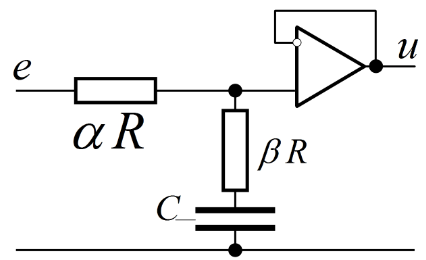
\includegraphics[width=5cm]{интегрирующая.png}
    \caption{Пропорционально интегрирующее звено.}
    \label{integr}
    \end{minipage}
    \hfill
    \begin{minipage}[h]{0.45\linewidth}
        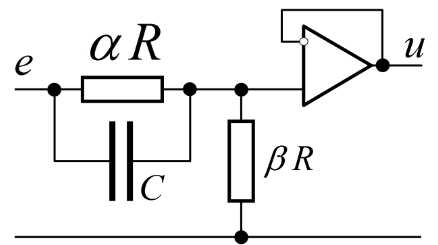
\includegraphics[width=5cm]{дифференцирующая.png}
        \caption{Пропорционально дифференцирующее звено.}
        \label{differ}
    \end{minipage}
    \end{center}
    \end{figure}

\begin{enumerate}
    \item Измерим уровни подавления на частоте $f_0$ и в полосах задержания для пропорционального интегрирующей и дифференцирующей цепей 
    с полюсом в точке $s = \frac{p}{\omega_0} = -1, f_0 = \frac{\omega_0}{2\pi}$ и нулями в точках $s = -2, s = -\frac{1}{2}$.
    Измерим уровни подавления на частоте $f_0$ и в полосах задержания.

    \begin{equation}
        \delta = \frac{\beta}{\alpha + \beta} = \frac{1}{2} - уровень\; подавления\; в\; полосе\; задержания
    \end{equation}

    Подавление на частоте $f_0 = 10k$:

       $$ \frac{4}{5} - интегрирующее\; звено, \frac{1}{5} - дифференцирующее\; звено $$

    \item Измерим номиналы резисторов в схемах так, чтобы сохранив положения полюсов,
    переместить нули точки $s = -4, s = -\frac{1}{4}$ \\
    $\delta = \frac{1}{4}$ - уровень подавления в полосе задержания. Уровень подавления на частоте $f_0$: $\frac{1}{2}$ - интегрирующая, $\frac{3}{20}$ - дифференцирующая.
    \item Откроем модель integrator.cir реального интегратора с частотой единичного усиления $f_1 = \frac{1}{2\pi RC} = 10k$ и усилением $K = \frac{R_K}{R}$.
    
    \begin{figure}[H]
        \begin{center}
        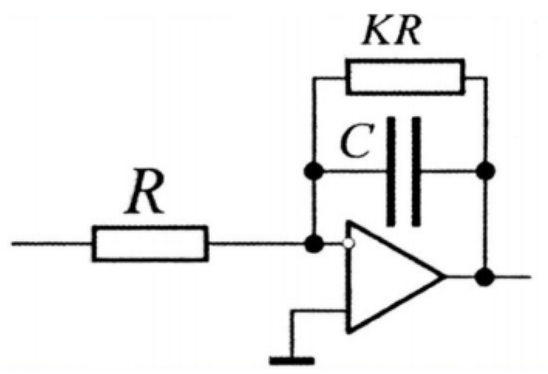
\includegraphics[width=6cm]{реальный_интегратор.png}
        \caption{Реальный интегратор.}
        \label{real} %% метка рисунка для ссылки на него
        \end{center}
    \end{figure}

    \begin{table}[H]
        \centering
        \begin{center}
        \end{center}
        \vspace{0.1cm}
        \label{tab:my_label}
        \begin{tabular}{ |p{2cm}|p{1cm}|p{1cm}|p{1cm}|p{1cm}|p{1cm}|p{1cm}|}
     \hline
     $f_1, Гц$ &  10k & 10k & 10k & 10k & 10k & 10k \\
    \hline
    K &  2 & 4 & 8 & 16 & 32 & 64 \\
    \hline
    $f_0, Гц$ &  5k & 2.5k & 1.25k & 0.61k & 0.31k & 0.15k \\
    \hline
    
    \end{tabular}
    \end{table}
    Соотношение $f_1 = f_0K$ - выполняется.
    
    \item Подключим step единичного перепада, изучим переходные характеристики интегратора $h_0(t/\tau_1)$, $\tau_1 = RC = 15.92\mu$.
    
    \begin{table}[H]
        \centering
        \begin{center}
        \end{center}
        \vspace{0.1cm}
        \label{tab:my_label}
        \begin{tabular}{ |p{2cm}|p{1.5cm}|p{3cm}|p{1.5cm}|p{2cm}|p{1cm}|p{1.3cm}|}
     \hline
    $t/\tau$ &  2 & 4 & 8 & 16 & 32 & 64 \\
    \hline
    $h$ &  0.82 & 1.62 & 3.22 & 6.42 & 12.82 & 25.63 \\
    \hline
    $h$ &   0.4  & 0.8 & 1.6 & 3.3 & 6.5 & 13.1 \\
    \hline

    \end{tabular}
    \end{table}
    Подключим источник pulse, проанализируем результаты интегрирования серии прямоугольных импульсов.

    \begin{table}[H]
        \centering
        \begin{center}
        \end{center}
        \vspace{0.1cm}
        \label{tab:my_label}
        \begin{tabular}{ |p{2cm}|p{1.5cm}|p{3cm}|p{1.5cm}|p{2cm}|p{1cm}|p{1.3cm}|}
     \hline
    $t/\tau$ &  2 & 4 & 8 & 16 & 32 & 64 \\
    \hline
    $h$ &  0.42 & 0.83 & 1.6 & 3.3 & 6.5 & 13.1 \\
    \hline
    \end{tabular}
    \end{table}
     

\end{enumerate}

\section{Задание №2. Активные звенья с двойным Т-мостом.}

\begin{figure}[H]
    \begin{center}
    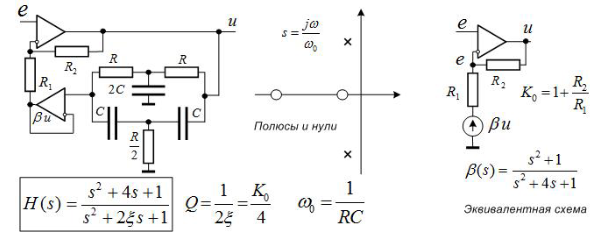
\includegraphics[width=12cm]{полосовой_фильтр.png}
    \caption{Полосовой фильтр с двойным Т-мостом.}
    \label{line} %% метка рисунка для ссылки на него
    \end{center}
\end{figure}

\begin{enumerate}
    \item Откроем модель полосовго фильтра pass2T.cir с $f_0 = 10k, K_0 = 20$. Измерим усиление на частоте $f_0$ и полосу $\varDelta f$ по уровню -3dB. 
    \\ Получили усиление $K_0 = 20.92, \varDelta f = 1/93 (R_2 = 20k)$.

    \begin{table}[H]
        \centering
        \begin{center}
        \end{center}
        \vspace{0.1cm}
        \label{tab:my_label}
        \begin{tabular}{ |p{2cm}|p{1.5cm}|p{3cm}|p{1.5cm}|p{2cm}|}
     \hline
    $R_2, Ом$ &  40k & 60k & 80k & 100k \\
    \hline
    $K_0 $ &  40.45 & 59.21 & 76.91 & 93.33 \\
    \hline
    $\varDelta f, Гц$ & 1038 & 698 & 547 & 461 \\
    \hline
    \end{tabular}
    \caption{Зависимость пикового усиления и ширины полосы от $R_5$.}
    \end{table}
     
    \item  Изучим поведение фильтра при разбалансировании моста варьированием $R_5$. Снимам зависимость пикового усиления.
    
    \begin{table}[H]
        \centering
        \begin{center}
        \end{center}
        \vspace{0.1cm}
        \label{tab:my_label}
        \begin{tabular}{ |p{2cm}|p{1cm}|p{1cm}|p{1cm}|p{1cm}|p{1cm}|p{1cm}|p{1cm}|p{1cm}|p{1cm}|}
     \hline
    $R_5, Ом$ &  1.5 & 2 & 2.5 & 3 & 3.5 & 4 & 4.5 & 5 & 5.5 \\
    \hline
    $K_0 $ &  32.46 & 43.77 & 79.67 & 956.78 & 90.59 & 42.88 & 28.13 & 21.01 & 16.85 \\
    \hline
    \end{tabular}
    \caption{Зависимость пикового усиления от $R_5$.}
    \end{table}

    \item Измерим уровни скачка в нуле и первого выброса: уровень скачка - 0.96В. 
    
    \begin{table}[H]
        \centering
        \begin{center}
        \end{center}
        \vspace{0.1cm}
        \label{tab:my_label}
        \begin{tabular}{ |p{2cm}|p{1cm}|p{1cm}|p{1cm}|p{1cm}|p{1cm}|p{1cm}|}
     \hline
    $R_5, Ом$ &  5k & 4.5k & 4k & 3.5k & 3k & 2.5k \\
    \hline
    Выброс &  4.29 & 4.49 & 4.72 & 5.01 & 5.36 & 5.82 \\
    \hline
    \end{tabular}
    \caption{Оценка значения $R_5$, при котором фильтр теряет устойчивость.}
    \end{table}
    Потеря устойчивости происходит при $R_5 = 3k Ом$.

    \item Откроем модель stop2T.cir с $f_0 = 10k, \gamma = 0.1$.
    
    \begin{figure}[H]
        \begin{center}
        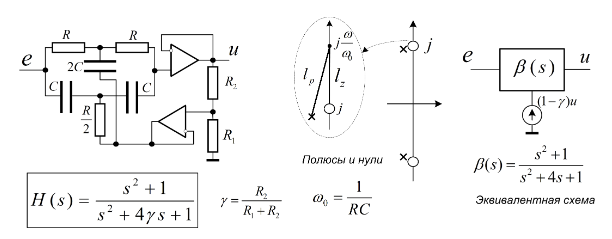
\includegraphics[width=12cm]{режекторный.png}
        \caption{Режекторный фильтр с двойным Т-мостом.}
        \label{regekt} %% метка рисунка для ссылки на него
        \end{center}
    \end{figure}
    Измерим ширину полосы режекции $\varDelta f$ по уровню 0.7 = -3dB. Получим: $\varDelta = 4.06k$Гц. \\
    Изучим ее изменение при варьировании $R_1$ и поведение фильтра при разбалансировании моста варьированием $R_5$.
    \item Изучим уровни скачка в нуле и первого выброса. Уровень скачка: 1В;первый выброс - 701.2мВ.  
\end{enumerate}

\section{Задание №3. Исследование созвездий.}

\begin{enumerate}
\item $n = 7, \; \varepsilon = 1, \; \eta = 2, \; \rightarrow \; \eta_1 = 5042$ - уровень затухания фильтра Чебышева,
тот же уровень затухания достигается фильтром Баттерворда порядка $n = 7$ при $\eta = 3.3808$

\item $n = 7, \; \varepsilon = 1, \; \eta = 1.5, \; \rightarrow \; \eta_1 = 421.5$ - уровень затухания фильтра Чебышева, порядок филтра Баттерворда с тем же затуханием
при $\eta = 1.5 \; \rightarrow \; \eta = 13$

\item Уровень затухания эллиптического фильтра при $n = 7, \; \varepsilon = 1, \; \eta = 1.1 \rightarrow \eta_1 = 608.46$.
При селективности $\eta = 1.56$ достигается тот же уровень затухания филтром Чебышева $n = 7, \; \varepsilon = 1$

\item Полосовой фильтр с частотой $f_0 = 465k$, двусторонней полосой $\Delta f = 24 k \; (Q = \frac{f_0}{\Delta f} \approx 20)$,
неравномерностью $3dB\; (\varepsilon = 1)$ и затуханием $\eta_1 = 10^4 = 80 dB$. Селективность $\eta = 1.36$
обеспечивает затухание $\eta_1$ эллиптическим фильтром порядка $n = 7$. При $n =2$ фильтр Чебышева обеспечивает сопоставимое значение селективности при том же
затухани. Преобразовав эти фильтры в полосовые с $Q = 20$ получаем максимальные добротности полюсов: $Q_{max} = 1049.39$ для эллиптического и $Q_{max} = 2084.96$ для
фильтра Чебышева.

\end{enumerate}


\graphicspath{ {pictures/} }

\section{Задание №4. Звенья Саллена-Ки.}


\begin{figure}[H]
    \begin{center}
        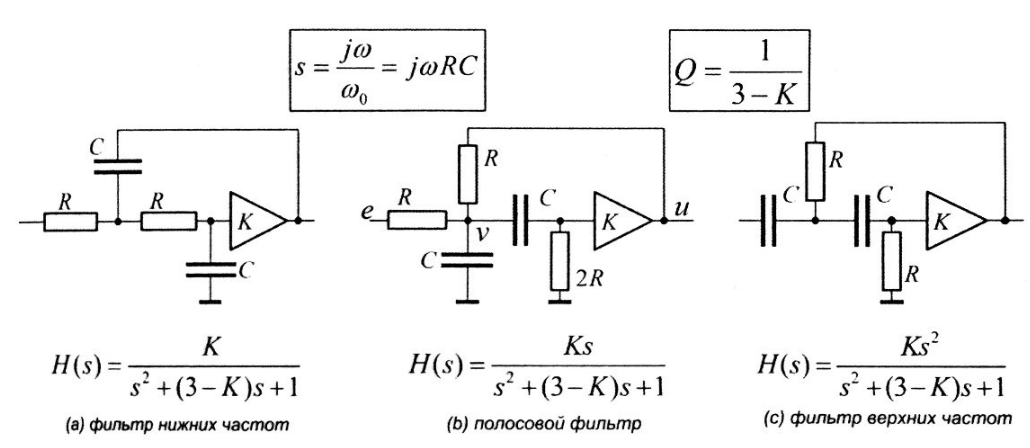
\includegraphics[scale = 0.6]{pic4.png}
        \caption{Звенья Саллена-Ки}
        \label{Sallen-Ki}
    \end{center}
\end{figure}

\begin{enumerate}
    \item Откроем \textbf{skey.cir} звеньев Саллена-Ки с частотой $f_0 = 10k$ и добротностью $Q=1$.
    Измерим значения кожффициентов передачи при $f= f_0$. Получим:
    $$K_0=2,\;\;K_{lp} = 27.6,\;\; K_{hp} = 27.53,\;\; K_{bp} = 27.6$$
    \item Откроем модель \textbf{sk3pole.cir} с фильтром Баттерворда верхних и нижних частот порядка $n = 3$
    на частоту среза $f_0 = 10k$. Измерим скорости спада в $dB$ на октаву и затухания на частотах $f_0/2, \; 2f_0$: \par 
    ВЧ: затухания на $f_0/2: \; -18\; dB,$ скорость спада $-18 \frac{dB}{дек}$ \par 
    НЧ: затухания на $2f_0: \; - 18.2\; dB,$ скорость спада $15 \frac{dB}{дек}$ \par 

    \ 

    % Измерим уровни затухания с фильтрами Чебышева на частотах $f_0/2, \; 2f_0$: \par 
    % ВЧ: затухания на $f_0/2: \; -30\; dB,$ скорость спада $-18 \frac{dB}{дек}$ \par 
    % НЧ: затухания на $2f_0: \; - 30\; dB,$ скорость спада $18 \frac{dB}{дек}$ \par 
\end{enumerate}

%     \item[4.] Откроем прототип \textbf{sk4pole.cir}, реализуем 4-полюсной полосовой фильтр Чебышева с $f_0 = 1k, \; \varepsilon = 1, \; Q = \frac{f_0}{\Delta f} = 6.$
%     Измерим затухание на частотах $f_0/2, 2f_0, f_0/10, 10f_0.$

%     \begin{table}[H]
%         \centering
%         \label{t1}
%         \vspace{0.1cm}
%         \begin{tabular}{|c||c|c|c|c|}
%      \hline
%     f & $f_0/2$ & $2f_0$& $f_0/10$& $10f_0$ \\
%     \hline
%     Затухание& & & &   \\
%     \hline
%     \end{tabular}
%     \end{table}
% \end{itemize}




% \section{Задание №5. Звенья с двойной обратной связью.}

% \begin{itemize}

%     \item[1.] полосовое звено с $f_0k, \; K_0 = 5,\; Q = 15$

%     $f_{max} = 4.980k, \; \Delta f = 338$ - ширина полосы по уровню 0.7.
%     $Q = \frac{f_{max}}{\Delta f} = 14.7, \; QK_0 = 73.5$ - пиковое усиление.

%     Построим график зависимости частоты пика от $R_2$

%     \begin{table}[H]
%         \centering
%         \label{t2}
%         \vspace{0.1cm}
%         \begin{tabular}{|c||c|c|c|c|c|c|c|}
%      \hline
%     $R_2$& 100& 300&500 &700 &900 &1100 &1300  \\
%     \hline
%     f & & & & & & &  \\
%     \hline
%     \end{tabular}
%     \end{table}

%     \begin{figure}[H]
%         \begin{center}
%             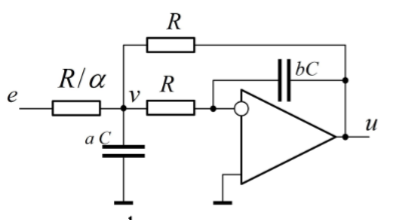
\includegraphics[scale = 0.6]{pic5.png}
%         \end{center}
%     \end{figure}

%     \item[3.] $C^* = \nu_1 = 11.63 \; нФ,\; R^* = R/\nu_2 = 8.61\;кОм$. Затухания:
    
%     \begin{table}[H]
%         \centering
%         \label{t3}
%         \vspace{0.1cm}
%         \begin{tabular}{|c||c|c|c|}
%      \hline
%     f& 0.5k&2k & 10k \\
%     \hline
%     Затухания & & &   \\
%     \hline
%     \end{tabular}
%     \end{table}

% \end{itemize}





% \section{Задание №6. Полосовое звено на сдвоенном усилителе.}

% \begin{figure}[H]
%     \begin{center}
%         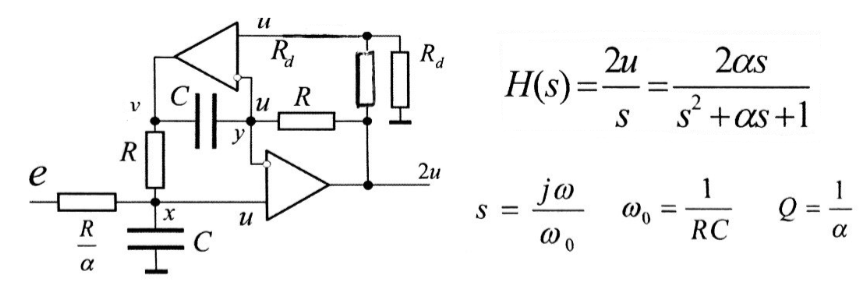
\includegraphics[scale = 0.6]{pic6.png}
%         \caption{Полосовой фильтр на сдвоенном операционном усилителе}
%         \label{pic6}
%     \end{center}
% \end{figure}

% \begin{itemize}
%     \item[1.] Откроем модель \textbf{amp2bp.cir}. По частотной характеристике звена оченим его параметры: 
%     $f_0 = 10k, \; Q = 9.7$. Измерим значение добротности при $R_2 = 6400k.$

%     \item[2.] Измерим частоту и уровень пика при $R_5 = 1.11k\; (\gamma = \frac{R_5}{R_4 + R_5} = 0.1): \; f = 31.415k,$
%     уровень пика - 24.079. 
% \end{itemize}



% \section{Задание №7. Звенья эллиптических фильтров.}

% \begin{enumerate}
%     \item Реализуем трехполюсной эллиптический фильтр нижних частот с параметрами $\eta = 1.5, \; f_0 = 1k, \; \varepsilon = 1,\; \eta_1 = 35.61, \; \nu_z = 1.67512,\; \nu_0 0.34797, \; \nu_p = 0.94016$, 
%     затухание - $31.03 \; dB$. \par 
%     Измерим границу $\eta$ полосы задержания, положение нуля и уровень затухания $\eta_1$:
%     $$\varepsilon = 0.64\; -\; неравномерность, \; \eta = 1.478k \; -\; граница\; полосы \;задержания$$
%     $$\eta_1 = 3.16 \; - \; уровень \;затухания,\; положение\; нуля: \;1.672k$$

%     % \begin{figure}[H]
%     %     \begin{center}
%     %         \includegraphics[scale = 0.6]{}
%     %         \caption{АЧХ и ФЧХ фильтра нижних частот}
%     %         \label{}
%     %     \end{center}
%     % \end{figure}


%     \item  Реализуем фильтр верхних частот с теми же параметрами. Измерим границу $\eta$ полосы задержания, положение нуля и уровень затухания.
%     $$\varepsilon = 0.59, \; \eta = 663.68, \eta_1 = 10.04$$

%     % \begin{figure}[H]
%     %     \begin{center}
%     %         \includegraphics[scale = 0.6]{}
%     %         \caption{АЧХ и ФЧХ фильтра верхних частот}
%     %         \label{}
%     %     \end{center}
%     % \end{figure}
%\end{enumerate}

\end{document}